\section{La Naturaleza del Engaño}
La psicología social define el engaño como: "\textit{el intento deliberado de un comunicador de fomentar una creencia o comprensión en otros que el receptor considera falsa}" (Vicianova M., 2015). Del mismo modo, los diccionarios utilizan estas mismas características para definir la mentira y el engaño. Por ejemplo, según la \textit{Real Academia Española}, el engaño es "\textit{una declaración que se desvía de la verdad o la pervierte}". El engaño es omnipresente, y algunos dirían que es un fenómeno necesario en la comunicación humana, pero su misma acción despierta la indignación moral y la rabia dentro de las personas (Vicianova M., 2015). 

La detección de mentiras es parte de numerosas profesiones criminales, médicas y legales (Vicianova M., 2015). Por extraño que suene, la mentira forma parte de la vida cotidiana de varias personas. Los agentes de policía se enfrentan al engaño, especialmente en la determinación de los hechos en los crímenes que se han cometido. Los jueces y abogados buscan justicia en las disputas legales y los especialistas médicos exigen la verdad para un diagnóstico preciso y un tratamiento adecuado de los pacientes. (Vicianova M., 2015)

Existe una brecha muy estrecha entre lo que se considera engañar a una persona o no, desde una perspectiva de segunda persona (Ekman P., 2009). Todas las personas se han enfrentado en su vida, sin lugar a duda, a una persona cuyas intenciones han sido las de ocultar la verdad. Y aun más allá de eso, toda persona en algún momento ha ocultado la verdad a alguien más. Pero no todas las situaciones le permiten al mentiroso enmascarar su auténtico sentir: hay mentiras que exigen ocultar las emociones sin inventar otras en su lugar, que es algo mucho más arduo todavía (Ekman P., 2009). Esto, entre muchos otros factores de distinto tipo, hacen que la complejidad en la detección de una mentira se eleve.

Para ocultar una emoción cualquiera, puede inventarse cualquier otra emoción falsa. La más habitualmente utilizada es la sonrisa (Ekman P., 2009). Actúa como lo contrario de todas las emociones negativas: temor, ira, desazón, disgusto, etc. Suele elegírsela porque para concretar muchos engaños el mensaje que se necesita es alguna variante de que uno está contento. Otro de los motivos por los cuales la sonrisa goza de tanta popularidad como máscara es que constituye la expresión facial de las emociones que con mayor facilidad puede producirse a voluntad (Ekman P., 2009). En efecto, existen varias técnicas para ocultar estas emociones humanas. Por ejemplo, otra técnica parecida consiste en decir la verdad de una manera retorcida, de tal modo que la víctima no la crea (Ekman P., 2009).

Por otro lado, la pista sobre una mentira, un embuste o la auto delación puede presentarse en un cambio de la expresión facial, un movimiento del cuerpo, una inflexión de la voz, el hecho de tragar saliva, un ritmo respiratorio excesivamente profundo o superficial, largas pausas entre las palabras, un desliz verbal, una micro expresión facial, un ademán que no corresponde (Ekman P., 2009). No siempre los mentirosos prevén en qué momento necesitarán mentir; no siempre tienen tiempo de preparar el plan que han de seguir, ensayarlo y memorizarlo. Aun cuando el mentiroso tenga la oportunidad de prepararse por adelantado y de montar cuidadosamente sus planes, tal vez no sea lo bastante sagaz como para anticipar todas las preguntas que pudieran hacerle o para meditar sus respuestas (Ekman P., 2009).

En sus formas más moderadas, este temor puede ayudar al mentiroso a no incurrir en equivocaciones al mantenerlo alerta. Si el temor es mayor, puede producir signos conductibles que el descubridor de mentiras avanzado notará enseguida; y si es mucho mayor, el temor del mentiroso a ser atrapado da origen exactamente a lo que él teme (Ekman P., 2009). Sin embargo, si alguien presenta una descripción falsa de lo que ha ocurrido en realidad, ello no significa necesariamente que esa persona intente engañar, y si no existe un intento deliberado de engañar, una afirmación falsa no se debe considerar una mentira (Ekman P., 2009).

Estos factores presentados, entre muchos otros, hacen que la detección del engaño sea una tarea compleja de realizar. En efecto, la motivación que puede tener una persona para mentir puede ser muy variada. Por medio de estudios realizados de manera independiente, se han podido identificar algunos motivos principales que pueden ser la causa para que un individuo mienta. Claro está que estos motivos no son los únicos que pueden existir. A continuación se listan los motivos principales que pueden motivar el engaño (Ekman P., 2009):

\begin{enumerate}
\item Evitar el castigo. Éste es el motivo más mencionado por los niños y los adultos. El castigo puede deberse a una mala acción o a un error involuntario. 
\item Para obtener una recompensa que no sería fácil conseguir de otra forma. Éste es el segundo motivo que tanto los niños como los adultos mencionan con más frecuencia. 
\item Para proteger de un castigo a otra persona. 
\item Para protegerse uno mismo de la amenaza de un daño físico. Esto es diferente del castigo, porque la amenaza de daño físico no se debe a una mala acción. Un ejemplo sería el niño que se encuentra solo en casa y que le dice a un desconocido que llama a la puerta que vuelva después porque su padre está descansando. 
\item Para ganarse la admiración de los demás. 
\item Para librarse de una situación social incómoda. Algunos ejemplos son el inventar una escusa para poder escapar de una reunión aburrida o terminar una conversación telefónica diciendo que llaman a la puerta. 
\item Para evitar la vergüenza. 
\item Para mantener la intimidad, sin dar a  conocer la intención de guardar en secreto cierta información. 
\item Para tener poder sobre otras personas controlando la información que les llega.
\end{enumerate}

En efecto, un mentiroso debe poner cuidado en elaborar precisamente y memorizar su falso plan (Ekman P., 2009). La mayoría de las personas que mienten no prevén todas las preguntas que pueden ser formuladas, ni todos los incidentes inesperados que pueden tener que enfrentar. Debe tener preparadas y ensayadas las respuestas ante un mayor número de contingencias de las que le gustaría afrontar. Inventar sobre la marcha de manera rápida y convincente, con una respuesta coherente con lo dicho y que pueda sostenerse en el futuro. Esto requiere una aptitud mental y una frialdad ante las situaciones tensas que pocos individuos poseen. Sin lugar a dudas, resulta muy difícil mentir sin cometer errores (Ekman P., 2009).

\section{El Cerebro Humano y la Actividad Emocional}
A lo largo del tiempo, y sobre todo en las décadas más recientes, se ha explorado activamente las funciones cerebrales y sus repercusiones en las actividades humanas más comunes. Sin embargo, estos acercamientos se han limitado a las ejecuciones cognitivas y volitivas de éste (James W., 1985). El centro de origen y procesamiento de las emociones se elude dentro del cerebro humano desde hace ya mucho tiempo. A pesar de esto, en lo concerniente a las emociones, incluso hoy es evidente que una de estas dos alternativas debe ser verdadera: ó bien su localización en el cerebro corresponde a centros independientes y especiales que únicamente tienen que ver con ellas, o bien corresponde a procesos que se dan en los centros motores y sensoriales ya designados o en otros de igual naturaleza aún no localizados (James W., 1985).

Son muchas las emociones que podemos experimentar los seres humanos. Algunas han sido llamadas emociones  ‘\textit{primarias}’, como son el miedo, la ira, la alegría, la tristeza, el disgusto y la sorpresa. Emociones que  van  acompañadas de patrones de conducta tales como respuestas faciales, motoras, vocales, endocrinas y autonómicas hasta cierto punto estereotipadas y que son reconocibles por encima de diferencias culturales y raciales en los seres humanos (Belmonte C., 2007). Estas emociones no desaparecen al momento de decir una mentira. Por el contrario, el engaño despierta muchas emociones en el individuo que pueden no pasar desapercibidas.

Por consiguiente, lo que llamamos coloquialmente ‘\textit{emoción}’ no se corresponde con un proceso cerebral separado e independiente, sino el resultado de múltiples mecanismos cerebrales que pueden  ser  distintos en emociones diferentes. Algo análogo a lo que ocurre  con  la  '\textit{memoria}’ o la  '\textit{inteligencia}’. En tal sentido, debe  tenerse  en  cuenta  también  que  los  componentes conscientes de las emociones,  que  denominamos  ‘\textit{sentimientos}’,  como  la  alegría,  el  miedo  o  el amor,  no  son  cualitativamente  diferentes  de  las  percepciones  cognitivas  como  podrían  ser  la  resolución de un problema matemático o la percepción de que el objeto en el que viajamos es un automóvil. Los mecanismos  de  procesamiento  inconsciente  que  subyacen en  ambos  casos  son  diferentes, pero en los dos, la consciencia se produce cuando el mecanismo cerebral general del conocimiento consciente los capta e incluye en su función (Belmonte C., 2007). Esto sugiere que las emociones humanas son procesos que se dan dentro del cerebro humano, tal y como lo puede ser cualquier otra actividad cerebral. De esta forma, las emociones que produce el engaño en un individuo, de alguna manera pueden de localizarse en el cerebro de igual manera.

La participación del lóbulo frontal, concretamente de la corteza \textit{frontomedial}, en el desarrollo de las conductas  emocionales, se conocía  desde  hace ya varios años a partir de experimentos independientes. La distribución de los diferentes elementos de la emoción entre ambos hemisferios cerebrales no es simétrica (Belmonte C., 2007). Por ejemplo, el hemisferio cerebral derecho está implicado en la comprensión y expresión de los aspectos afectivos del lenguaje y los elementos corporales de la expresión emocional. De modo que la mitad izquierda del cuerpo, que es la que controla  este  hemisferio,  expresa  las  emociones en mayor medida y esto se pone en evidencia porque los músculos de ese lado de la cara, reflejan en grado más contundente la emoción que la mitad derecha de ésta (Belmonte C., 2007). Por otra parte, los pacientes con lesiones en el hemisferio izquierdo pierden en cierto grado la capacidad  de  experimentar sentimientos  positivos  y  en  ellos  los  cuadros  depresivos son mucho más graves (Belmonte C., 2007).

Como resultado a estos estudios, en la actualidad, se ha eludido la relación entre la estructura del cerebro humano con funciones humanas. De igual manera, se elude la relación entre patrones de actividad neuronal con actividades del ser humano (Davatzikos et al., 2005). El análisis de patrones cuantitativos en el espacio-tiempo de la actividad cerebral conlleva a un análisis multivariable, poco explorado a principios de siglo por la limitación del procesamiento de datos de aquel entonces. El uso de algoritmos de Aprendizaje de Máquina para clasificar complejos patrones de activación cerebral se ha empezado a abordar en diversos estudios (Davatzikos et al., 2005).

\section{Del Polígrafo a la Detección de Mentiras Basada en el Cerebro}
En 1881, el primer dispositivo moderno de detección de mentiras llamado \textit{Guante de Lombrosso} fue creado por el criminólogo, médico y antropólogo italiano Cesare Lombrosso. Intentó medir los cambios en la presión arterial de la persona acusada, que se registraron en un gráfico o tabla. Esta sofisticada tecnología fue mejorada durante la Primera Guerra Mundial por William M. Marston y fue elaborada en su versión final después de la guerra. Este dispositivo sirvió para registrar los cambios en la presión arterial y los cambios en la respiración mientras se daba testimonio (Vicianova M., 2015).  

Dado el hecho de que los estudios señalan la relación entre la respiración torácica y la diafragmática como un indicador sensible de estrés y cambio emocional, los polígrafos modernos miden la frecuencia respiratoria del tórax y del abdomen por separado, lo que lleva a un aumento significativo en el valor diagnóstico de la medición. La base para evaluar el resultado de un polígrafo está en la relación entre los cambios fisiológicos que se manifiestan cuando una persona no está diciendo la verdad. Estos cambios pueden ser observados y medidos por el polígrafo utilizando la conductancia de la piel, la presión arterial, la frecuencia cardíaca y la respiración. Desafortunadamente, los cambios corporales pueden variar y también son producidos por estados diferentes a la mentira (Vicianova M., 2015).  

En efecto, se puede afirmar que el polígrafo no detecta mentiras, sino que mide las respuestas fisiológicas postuladas para ser asociadas con el engaño. Ninguna de estas respuestas son específicas al engaño, ni están necesariamente siempre presentes cuando ocurre el engaño. Sin embargo, cuando es usado por examinadores bien entrenados y en conjunción con otras técnicas, parece ofrecer un complemento útil para identificar a aquellos que intentan engañar (Vicianova M., 2015). 

Por otro lado, desde los años ochenta y el inicio de la neurociencia, han surgido puntos de vista completamente diferentes sobre la posibilidad de detectar mentiras al más alto nivel de los procesos mentales a través del medio de la medición de actividades cerebrales tales como la \textit{estimulación magnética transcraneal} (EMT), la \textit{resonancia magnética funcional} (IRMf), la \textit{tomografía por emisión de positrones} (RMN) y la \textit{toma de huellas dactilares cerebrales} (Onda de electroencefalográma, EEG). (Vicianova M., 2015).

En 2002, se describió el primer método de huellas dactilares cerebrales. La toma de huellas dactilares cerebrales es una forma de obtener información de una onda específica del electroencefalograma. La teoría es que el cerebro procesa la información conocida y relevante de manera diferente a como procesa la información desconocida o irrelevante (Vicianova M., 2015). El procesamiento por parte del cerebro de información conocida, como los detalles de un crimen almacenado en el cerebro, es revelado por un patrón específico en el electroencefalograma.

A pesar de los resultados, el método de tomar las huellas dactilares del cerebro presenta algunas desventajas. Para que estas técnicas sean útiles en la detección de mentiras, los investigadores deben tener suficiente información sobre el hecho y el autor del delito (Vicianova M., 2015). Esto es necesario para poder documentar los patrones de electroencefalograma sospechosos cuando se proporciona la respuesta correcta. Otros estudios publicados que examinan la función cerebral durante el engaño han demostrado que los resultados de estos métodos no son lo suficientemente precisos y carecen de una base empírica sólida (Wolpe et al., 2005). Se señala problemas con la replicación, grandes diferencias cerebrales individuales y regiones cerebrales no especificadas asociadas con el decir la verdad. Además, la actividad cerebral al mentir depende de la situación. 

Otra limitación de las técnicas en el campo de la detección de mentiras es el propio cerebro humano. Procesa todo lo que pasa a través del campo perceptivo no sólo desde afuera, sino también desde adentro. Es irrelevante hasta qué punto esta actividad penetrará en la conciencia. La acusación, con razón o sin ella, lleva al cerebro al límite de la situación: dinamiza la memoria, la atención, el nivel emocional y la capacidad de tomar decisiones. Todos estos cambios pueden ser registrados usando resonancia magnética funcional o a través de un polígrafo. Sin embargo, es posible "ocultar" lo que ocurre en el cerebro durante la solución de la tarea ocupando el cerebro con actividades completamente diferentes (por ejemplo, operaciones matemáticas o recuerdos), una técnica llamada defensa personal (Vicianova M., 2015).

De igual manera, otro problema surge de experimentos que son puramente de laboratorio y los participantes son en gran medida una muestra específica. Sus resultados pueden no corresponderse con los resultados de otros grupos de prueba. De manera similar, surge el hecho de que se pide a los experimentadores que engañen, por lo que no se considera una mentira espontánea. La posibilidad de evitar esto sería no seguir instrucciones. El experimentador debe intervenir sólo si el participante lo solicita. Igualmente, otro problema se refiere a la diversidad de situaciones y con diferentes tipos de engaño. Diferentes personas con el mismo tipo de fraude pueden tener un tipo de actitud diferente. Por lo tanto, la personalidad y la actitud de un individuo deben ser tenidas en cuenta.

La detección del engaño y la confirmación de la verdad con la poligrafía convencional ha planteado una serie de problemas técnicos y éticos (Wolpe et al., 2010).  El análisis de señales electromagnéticas del cerebro se ha postulado como una alternativa viable para la detección de la mentira en ámbitos legales y profesionales. Incluso algunos métodos se promueven como más efectivos que el polígrafo convencional. Sin embargo, estos métodos aun poseen limitaciones en cuanto a la falta de exploración de los mismos y a la poca estandarización que se tiene en su campo de estudio (Wolpe et al., 2010). 

\section{Aprendizaje de Máquina}
Para resolver un problema en una computadora, necesitamos un algoritmo.  Un algoritmo es una secuencia de instrucciones finitas que se llevan a cabo a partir de una entrada, para brindar una salida. Por ejemplo, se puede crear un algoritmo para clasificar. La entrada es un conjunto de números y la salida es su lista ordenada. Para la misma tarea, puede haber varios algoritmos y puede que nos interese encontrar el más eficiente, que requiera el menor número de instrucciones o memoria o ambos. (Alpaydn E., 2014)

Para algunas tareas, sin embargo, no tenemos un algoritmo. Por ejemplo, para distinguir los correos electrónicos de \textit{spam} de los correos electrónicos legítimos. Sabemos lo que la entrada es: un documento de correo electrónico que, en el caso más simple, es un archivo de caracteres. Sabemos cuál debe ser la salida: una salida "sí" o "no" que indique si el mensaje es spam o no.  No sabemos cómo transformar la entrada en salida. Lo que se puede considerar spam cambia con el tiempo y de persona a persona.(Alpaydn E., 2014)

Lo que nos falta de conocimiento, lo compensamos con datos. Podemos compilar fácilmente miles de mensajes de ejemplo, algunos de los cuales sabemos que son spam y lo que queremos es "aprender" lo que significa spam de ellos. En otras palabras, queremos que una máquina, una computadora, extraiga automáticamente el algoritmo para esta tarea.  No hay necesidad de aprender a ordenar números, ya tenemos algoritmos para ello; pero hay muchas aplicaciones para las que no tenemos un algoritmo pero sí tenemos datos de ejemplo.(Alpaydn E., 2014) Pero el aprendizaje automático no es sólo un problema de base de datos; también es parte de la inteligencia artificial.  Para ser inteligente, un sistema que se encuentra en un entorno cambiante debe tener la capacidad de aprender. Si el sistema puede aprender y adaptarse a estos cambios, el diseñador del sistema no necesita prever y proporcionar soluciones para todas las situaciones posibles.

El aprendizaje automático consiste en programar máquinas, computadoras, para optimizar un criterio de rendimiento utilizando datos de ejemplo o experiencias pasadas. Tenemos un modelo definido hasta algunos parámetros, y el aprendizaje es la ejecución de un programa informático para optimizar los parámetros del modelo utilizando los datos de la formación o la experiencia pasada. El modelo puede ser predictivo para hacer predicciones en el futuro, o descriptivo para obtener conocimiento de los datos, o ambos. El aprendizaje automático utiliza la teoría de la estadística en la construcción de modelos matemáticos, porque la tarea principal es hacer inferencias a partir de una muestra.  

Computacionalmente, hay dos vertientes principales respecto a estos algoritmos. Primero, en el entrenamiento, necesitamos algoritmos eficientes para resolver el problema de optimización, así como para almacenar y procesar la enorme cantidad de datos que generalmente tenemos. En segundo lugar, una vez que se aprende un modelo, su representación y solución algorítmica para la inferencia también debe ser eficiente. En ciertas aplicaciones, la eficiencia del algoritmo de aprendizaje o inferencia, es decir, su complejidad espacial y temporal, puede ser tan importante como su precisión predictiva (Alpaydn E., 2014).

El aprendizaje supervisado, en el contexto de la \textit{inteligencia artificial} (IA) y el aprendizaje automático, es un tipo de sistema en el que se proporcionan tanto los datos de entrada como los datos de salida deseados. Los datos de entrada y salida se etiquetan para su clasificación a fin de proporcionar una base de aprendizaje para el futuro procesamiento de datos. Los modelos de aprendizaje supervisado tienen algunas ventajas sobre el enfoque no supervisado, pero también tienen limitaciones. Es más probable que los sistemas emitan juicios con los que los seres humanos puedan relacionarse, por ejemplo, porque los seres humanos han proporcionado la base para las decisiones. Sin embargo, los sistemas de aprendizaje supervisado tienen problemas para manejar la nueva información. 
\begin{center}
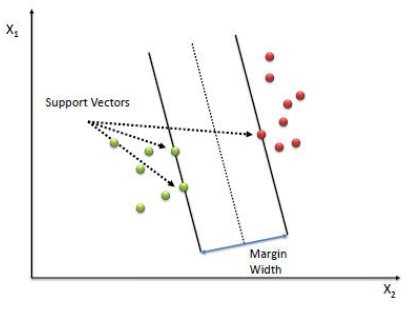
\includegraphics[height=2.0in]{figuras/Capture3.PNG}
\end{center}

Entre los algoritmos de aprendizaje de máquina, está la \textit{Máquina de Vectores de Soporte} (SVM en Inglés). Este algoritmo puede implementarse de varias maneras, de acuerdo a la naturaleza de la información que se le proporciona, y ha sido popular en los últimos años por una serie de razones (Alpaydn E., 2014): 
\begin{enumerate}
\item Es un método basado en la discriminación y utiliza el principio de \textit{Vapnik}, de nunca resolver un problema más complejo como primer paso antes del problema real. 
\item Después del entrenamiento, el parámetro del modelo lineal, el vector de peso, puede anotarse en términos de un subconjunto del conjunto de entrenamiento, que son los llamados vectores de apoyo. En la clasificación, estos son los casos que están cerca del límite y como tal, conocerlos permite la extracción del límite de conocimiento: son los casos inciertos o erróneos que se encuentran en las cercanías del límite entre dos clases.  
\item La salida se escribe como una suma de las influencias de los vectores de soporte y estas son dadas por las funciones del núcleo que son medidas específicas de la aplicación de similitud entre las instancias de datos. 
\item Típicamente en la mayoría de los algoritmos de aprendizaje, los puntos de datos se representan como vectores, y se utiliza tanto el producto de puntos como la distancia euclídea.  Una función del kernel nos permite ir más allá. 
\item Los algoritmos basados en el núcleo están formulados como problemas de optimización convexos, y hay un solo óptimo que podemos resolver analíticamente. Por lo tanto, ya no nos preocupa la heurística de los ritmos de aprendizaje, las inicializaciones, la comprobación de la convergencia, etc. Por supuesto, esto no significa que no tengamos ningún hiper-parámetro para la selección del modelo; cualquier método lo necesita, para hacer coincidir el algoritmo con los datos disponibles.
\end{enumerate}

\section{Máquina de Vectores de Soporte}

\begin{center}
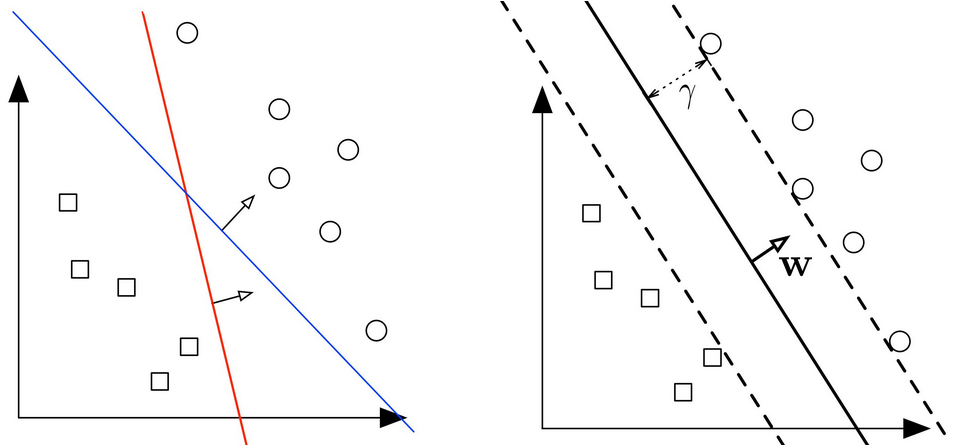
\includegraphics[height=2.0in]{figuras/Capture1.PNG}
\end{center}

\textit{Máquina de Vectores de Soporte} (SVM, por sus siglas en inglés) es un poderoso método de clasificación que encuentra la hiper-superficie que maximiza el margen entre dos distribuciones (Chih-Wei Hsu, Chih-Chung Chang, 2008), las respuestas verdaderas y no verdaderas en nuestro caso. El objetivo de un SVM es producir un modelo que predice los valores objetivo de un set de datos, a partir de únicamente los atributos del mismo set.  Formalmente, se describe como: dado un set de valores de la forma $(x_i,y_i), i=1, ..., l$  donde  $x_i \in R^n$ y $y\in\left\lbrace1,-1\right\rbrace^l$, el SVM (Boser, Guyon, \& Vapnik, 1992) requiere la solución al siguiente problema de optimización: 
\begin{center}
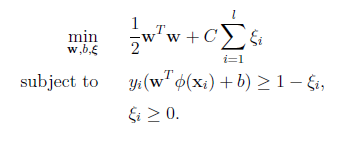
\includegraphics[height=1.15in]{figuras/Imagen1.png}
\end{center}
Los vectores de entrenamiento $x_i$ son mapeados en un espacio dimensional más alto por la función $\phi$. SVM busca un hiper-plano separador lineal con el máximo margen en este espacio dimensional. $C > 0$ es el parametro de penalidad en el término de error. Consecuentemente, $K(x_i,x_j)\equiv \phi(x_i )^T \phi(x_j)$ se conoce como la función kernel. Cada vez más, nuevas funciones kernel son propuestas por investigadores. Algunas conocidas son los kernel \textit{lineal}, \textit{polinomial}, \textit{función de base radial} (RBF) y \textit{sigmoid} (Chih-Wei Hsu, Chih-Chung Chang, 2008). 

\begin{itemize}
\item Linear: $K(x_i,x_j ) = x_i^Tx_j$
\item Polinomial: $K(x_i,x_j ) = (\gamma x_i^Tx_j + r)^d$,$\gamma > 0$
\item Radial Basis Function (RBF): $K(x_i,x_j ) = exp(-\gamma \norm{x_i-x_j}^2)$,$\gamma>0$
\item Sigmoid: $K(x_i,x_j ) = tanh(\gamma x_i^Tx_j + r)$
\end{itemize}

Donde $\gamma$, $r$ y $d$ son parámetros de kernel.  

En general, el núcleo RBF es una primera opción razonable al momento de implementar este tipo de algoritmo. Este núcleo no lineal mapea muestras en un espacio dimensional más alto, por lo que, a diferencia del núcleo lineal, puede manejar el caso cuando la relación entre las etiquetas de clase y los atributos es no lineal.  Además, el núcleo lineal es un caso especial de RBF, ya que el núcleo lineal con un parámetro de penalización $C$ tiene el mismo rendimiento que el núcleo RBF con algunos parámetros ($C$,$\gamma$).  Además, el núcleo sigmoide se comporta como RBF para ciertos parámetros. La segunda razón es el número de hiper-parámetros que influyen en la flexibilidad de la selección del modelo.  El núcleo polinomial tiene más hiper-parámetros que el núcleo RBF. Finalmente, el núcleo RBF tiene menos dificultades numéricas. Sin embargo, hay algunas situaciones en las que el núcleo RBF no es adecuado. En particular, cuando el número de características es muy grande, se puede usar el kernel lineal (Chih-Wei Hsu, Chih-Chung Chang, 2008).

Hay dos parámetros para un kernel RBF: $C$ y $\gamma$  No se sabe de antemano qué $C$ y $\gamma$ son los mejores para un problema determinado, por lo que se debe realizar algún tipo de selección de modelo.  El objetivo es identificar el mejor ($C$,$\gamma$) para que el clasificador pueda predecir con precisión los datos desconocidos (es decir, los datos de las pruebas) (Chih-Wei Hsu, Chih-Chung Chang, 2008).  Se debe de considerar que puede no ser útil para lograr una alta precisión de la formación. Es decir, un clasificador que prediga con precisión los datos de formación cuyas etiquetas de clase son realmente conocidas.  Como se mencionó anteriormente, una estrategia común es separar el conjunto de datos en dos partes, una de las cuales se considera desconocida.  

La precisión de la predicción obtenida a partir del conjunto "desconocido" refleja con mayor precisión el rendimiento de la clasificación de un conjunto de datos independiente.  Una versión mejorada de este procedimiento se conoce como validación cruzada. En la validación cruzada en $\upsilon$, primero dividimos el conjunto de entrenamiento en subconjuntos $\upsilon$ de igual tamaño.  Secuencialmente se prueba un subconjunto usando el clasificador entrenado en los subconjuntos $\upsilon$ - 1 restantes.  De este modo, cada instancia del conjunto de entrenamiento se predice una vez, de modo que la precisión de la validación cruzada es el porcentaje de datos que se clasifican correctamente. El procedimiento de validación cruzada puede evitar el problema de \textit{overfitting} (Chih-Wei Hsu, Chih-Chung Chang, 2008), es decir, que el modelo se ajuste demasiado a los datos, que nuevos valores de predicción desconocidos tengan un alto error respecto al modelo. 

\begin{center}
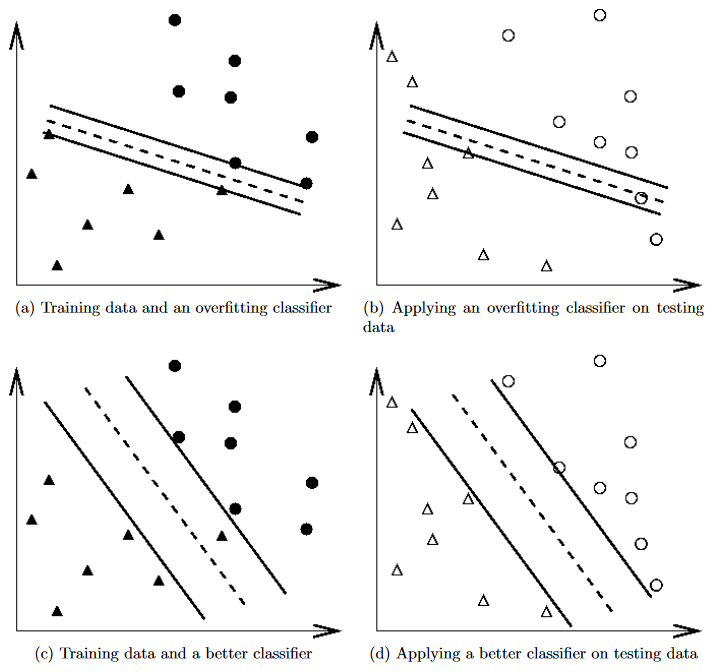
\includegraphics[height=5.15in]{figuras/Capture2.PNG}
\end{center}

En efecto, se recomienda un "\textit{grid-search}" en $C$ y $\gamma$ con validación cruzada.  Se prueban varios pares de valores ($C$,$\gamma$) y se escoge el que tenga la mejor precisión de validación cruzada. Probar secuencias de $C$ y $\gamma$ que crecen exponencialmente es un método práctico para identificar buenos parámetros (por ejemplo, $C$ = $2^(-5), 2^(-3), ..., 2^15$ $\gamma$ = $2^(-15), 2^(-13),..., 2^3$). Existen varios métodos avanzados que pueden ahorrar costes de cálculo, por ejemplo, aproximando la tasa de validación cruzada. Sin embargo, hay dos motivos por los que se prefiere el enfoque de búsqueda por cuadrícula simple. Una es que, psicológicamente, puede que no nos sintamos seguros al usar métodos que evitan hacer una búsqueda exhaustiva de parámetros por aproximaciones o heurística.   La otra razón es que el tiempo computacional requerido para encontrar buenos parámetros mediante la búsqueda en la cuadrícula no es mucho mayor que el de los métodos avanzados, ya que sólo hay dos parámetros. Además, la búsqueda en la red puede ser fácilmente paralelizada porque cada una ($C$,$\gamma$) es independiente (Chih-Wei Hsu, Chih-Chung Chang, 2008).

La información de la actividad cerebral y los patrones que se pueden extraer de la misma tiene una relación no lineal (Davatzikos et al., 2005). El kernel radial basis function (RBF) tiene utilidad cuando la información tiene esta característica. Este kernel asigna muestras de forma no lineal a un espacio dimensional superior para que, a diferencia del kernel lineal, pueda manejar el caso cuando la relación entre los valores objetivos y los atributos no es lineal. Una de las características más importantes de SVM es que no se calcula a partir de todas las muestras, sino sólo a partir de muestras que se encuentran cerca de la interfaz entre los dos grupos de interés. En nuestro caso, el algoritmo se centra sólo en los patrones de activación que son difíciles de clasificar en respuestas verídicas o no veraces (Davatzikos et al., 2005).

\section{Casos de Detección del Engaño a través de señales EEG por Medio de Algoritmos de Aprendizaje de Máquina}
Los rápidos avances en \textit{imagenología} médica diagnóstica en la última década han revolucionado la neurociencia. Los científicos están adquiriendo una nueva comprensión de la función y la estructura del cerebro, y están descubriendo ideas emocionantes y desafiantes sobre la naturaleza del comportamiento humano. Los avances en resonancia magnética, electroencefalografía, y otras técnicas modernas, pueden, por primera vez, medir de manera confiable los cambios en la actividad cerebral asociados con pensamientos, sentimientos y conductas, en principio permitiendo a los buscadores vincular los patrones de actividad cerebral directamente con los procesos o estados cognitivos o afectivos que producen. (Wolpe et al., 2010)

Varios estudios relacionados, sin embargo, han utilizado preguntas con respecto a memorias recientes y encontraron que las respuestas incorrectas (engañosas) resultaron en una activación significativa de las corticales bilaterales ventrolaterales prefrontales. Otro grupo que usó cartas de juego y un paradigma de conocimiento culpable encontró una activación significativa en la corteza cingulada anterior, el giro frontal superior y la corteza motora izquierda, premotora y parietal anterior. Otro grupo usó pares de sujetos con uno de ellos, dando periódicamente información engañosa a su pareja mientras eran escaneados. Durante los períodos de tiempo de cepa, encontraron un aumento de la actividad en las precorredencias laterales bilaterales prefrontales y motoras, la corteza parietal izquierda y la precuneta bilateral. La diversidad de paradigmas hace que cualquier conclusión sea muy difícil.(Revell et al., 2004)

La electroencefalografía no es más que un registro de la actividad eléctrica generada por el cerebro. El primer informe sobre la actividad eléctrica cerebral en humanos fue publicado en 1929, lo que permitió a los médicos y científicos observar el cerebro en acción de una manera significativa. Hay millones de neuronas en nuestro cerebro. Estas actividades generan millones de pequeños campos de tensión eléctrica.  La suma de estos campos de tensión puede ser detectada por electrodos colocados en el cuero cabelludo.  Por lo tanto, podemos decir que el EEG es la superposición de muchas señales más pequeñas.  La amplitud de estas señales oscila entre 1 $\mu V$ y 100 $\mu V$ en una persona normal. Las diferentes frecuencias eléctricas en el EEG pueden asociarse con diferentes acciones físicas y estados mentales[3]. Por lo tanto, el EEG muestra una amplia variación en la amplitud dependiendo de la estimulación externa y de los diferentes estados mentales internos. (Umale et al., 2016)

Estas señales pueden ser captadas usando varios equipos disponibles que generalmente consisten en electrodos que se colocan en el cuero cabelludo con un gel conductor entre los electrodos y el cuero cabelludo.  Los electrodos se colocan en diferentes posiciones del cuero cabelludo que captan las señales de diferentes partes del cerebro. Las señales de EEG sin procesar no pueden utilizarse directamente para la detección de tensiones. El pre-procesamiento es necesario para extraer características útiles que se pueden utilizar con varios algoritmos de aprendizaje de la máquina. (Umale et al., 2016)




